\documentclass{article}
\usepackage{bkc}
\usepackage{ccfonts}
\usepackage{tikz-cd}

\setassn{Math 6510 Problem Set 8}

\usetikzlibrary{decorations.markings,decorations.pathmorphing,matrix,arrows}
\tikzset{middlearrow/.style={
        decoration={markings,
            mark= at position 0.5 with {\arrow{#1}} ,
        },
        postaction={decorate}
    }
}

\newcommand{\im}{\text{im }}
\DeclareGraphicsExtensions{.pdf,.png,.jpg}
 
\begin{document}
\begin{exercise}{2.2.9}{\parindent}
  Compute the homology groups of the following 2-complexes:
  \begin{enumerate}
  \item The quotient of $S^2$ obtained by indentifying north and south
    poles to a point.
  \item $S^1 \times (S^1 \vee S^1)$.
  \item The space obtained from $D^2$ by first deleting the interios
    of two disjoint subdisks in the interior of $D^2$ and then
    identifying all three resulting boundary circles together via
    homeomorphisms preserving clockwise orientations of these circles.
  \item The quotient space of $S^1 \times S^1$ obtained by identifying
    points in the circles $S^1 \times \{x_0\}$ that differ by $2\pi/m$
    rotation and identifying points in the circle $\{x_0\} \times S^1$
    that differ by $2\pi/n$ rotation.
  \end{enumerate}
\end{exercise}
\begin{solution}{\parindent}
  TODO
\end{solution}

\begin{exercise}{2.2.10}{\parindent}
  Let $X$ be the quotient space of $S^2$ under the identifications $x
  \sim -x$ for $x$ in the equator $S^1$. Compute the homology groups
  $H_i(X)$. Do the same for $S^3$ with antipodal points of the
  equatorial $S^2 \subset S^3$ identified.
\end{exercise}
\begin{solution}{\parindent}
  TODO
\end{solution}

\begin{exercise}{2.2.12}{\parindent}
  Show that the quotient map $S^1 \times S^1 \to S^2$ collapsing the
  subspace $S^1 \vee S^1$ to a point is not nullhomotopic by showing
  that it induces an isomorphism on $H_2$. On the other hand, show via
  covering spaces that any map $S^2 \to S^1 \times S^1$ is
  nullhomotopic.
\end{exercise}

\begin{exercise}{2.2.14}{\parindent}
  A map $f: S^n \to S^n$ satisfying $f(x) = f(-x)$ for all $x$ is
  called an \textit{even map}. show that an even map $S^n \to S^n$
  must have even degree and that the degree must in fact be zero when
  $n$ is even. When $n$ is odd, show that there exist even maps of any
  given even degree.
\end{exercise}
\begin{solution}{\parindent}
  TODO
\end{solution}


\begin{exercise}{2.2.23}{\parindent}
  Show that if the closed orientable surgace $M_g$ of genus $g$ is a
  covering space of $M_k$, then $g = n(h-1) + 1$ for some $n$, namely,
  $n$ is the number of sheets in the covering.
\end{exercise}
\begin{solution}{\parindent}
  TODO
\end{solution}

\begin{exercise}{2.2.24}{\parindent}
  Suppose we build $S^2$ from a finite collextion of polygons by
  identifying edges in pairs. Show that in the resulting CW structure
  on $S^2$ the 1-skeleton cannot be either of the two graphs shown,
  with five and six vertices.
  \begin{center}
    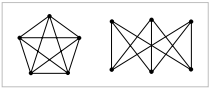
\includegraphics[scale=.7]{graphs.png}
  \end{center}
\end{exercise}
\begin{solution}{\parindent}
  TODO
\end{solution}

\begin{exercise}{2.2.28}{\parindent}
  \vspace*{-\bigskipamount}
  \begin{enumerate}
  \item Use the Mayer-Vietoris sequence to compute the homology groups
    of the space obtained from a torus $S^1 \times S^1$ by attaching a
    M\"{o}bius band via a homeomorphism from the boundary circle of
    the M\"{o}bius band to the circle $S^1 \times \{x_0\}$ in the
    torus.
  \item Do the same for the space obtained by attaching a M\"{o}bius
    band to $\R P^2$ via a homeomorphism of its boundary circle to the
    standard $\R P^1 \subset \R P^2$.
  \end{enumerate}
\end{exercise}
\begin{solution}{\parindent}
  TODO
\end{solution}

\begin{exercise}{2.2.31}{\parindent}
  Use the Mayer-Vietoris sequence to show there are isomorphisms
  $\tilde{H}_n(X \vee Y) \sim \tilde \tilde{H}_n(X) \oplus
  \tilde{H}_n(Y)$ if the basepoints of $X$ and $Y$ that are identified
  in $X \vee Y$ are deformation retracts of $U \subset X$ and $V
  \subset Y$.
\end{exercise}
\begin{solution}{\parindent}
  TODO
\end{solution}

\begin{exercise}{2.2.32}{\parindent}
  For $SX$ the suspension of $X$, show by a Mayer-Vietoris sequence
  applied to $X \cup CA$, where $CA$ is the cone on $A$.
\end{exercise}
\begin{solution}{\parindent}
  TODO
\end{solution}

\begin{exercise}{2.2.41}{\parindent}
  For a finite CW complex and $F$ a field, show that the Euler
  characterisitic $\capchi(X)$ can also be compute by the formula
  $\capchi(X) = \sum_n (-1)^n\dim H_n(X;F)$ the alternating sum of the
  dimensions of the vector spaces $H_n(X;F)$.
\end{exercise}
\begin{solution}{\parindent}
  TODO
\end{solution}

\begin{problem}{A1}{\parindent}
  Use Euler characteristic to determine which orientable surface
  results from identifying opposite edges of a $2n$-gon.
\end{problem}
\begin{solution}{\parindent}
  TODO
\end{solution}

\begin{problem}{A2}{\parindent}
  The degree of a homeomorphism $f: \R6n \to \R^n$ can be defined as
  the degree of the extension of $f$ to a homeomorphism of the
  one-point compactification $S^n$. Using this notion, fill in the
  details of the following argument which shows that $\R^n$ is not
  homeomorphic to a product $X \times X$ if $n$ is odd. Assuming $\R^n
  = X \times X$, consider the homeomorphism $f: \R^n \times \R^n \to X
  \times X \times X \times X$ that cyclically permutes the factors
  $f(x_1,x_2,x_3,x_4) = (x_2,x_3,x_4,x_1)$. Then $f^2$ switches the
  two factors of $\R^n \times \R^n$, so $f^2$ has degree $-1$ if $n$
  is odd. But $\deg(f^2) = \deg(f)^2 = 1$.
\end{problem}
\begin{solution}{\parindent}
  TODO
\end{solution}

\begin{problem}{A3}{\parindent}
  Show that if $f: \Delta^n \to \Delta^n$ is a map that takes each
  $(n-1)$-dimensional face of $\Delta^n$ to itself, then $f$ is
  surjective.
\end{problem}
\begin{solution}{\parindent}
  yer
\end{solution}

\begin{exercise}{A4}{\parindent}
  Show that the spaces $S^1 \times S^2$ and $S^1 \vee S^2 \vee S^3$
  have isomorphic homology and fundamental groups but are not homotopy
  equivalent.
\end{exercise}
\begin{solution}{\parindent}
  WEPA
\end{solution}
\end{document}